% Simple/short benchmark summary -- compile with tectonic.
\documentclass[11pt]{article}
\usepackage[margin=1in]{geometry}
\usepackage{amsmath,amssymb}
\usepackage{graphicx}
\usepackage{booktabs}
\usepackage{siunitx}
\usepackage[hidelinks]{hyperref}
\usepackage{caption}
\graphicspath{{figures/}}

\title{\textbf{Thin-walled MSG shell vs.\ 3D solid: benchmark summary}}
\author{Akshat Bagla \quad\small (Purdue University)}
\date{\today}

\begin{document}
\maketitle
\vspace{-2.5em}

\paragraph{What was tested.} The MSG thin-walled shell cross-sectional analysis,
in Reissner--Mindlin (RM, $C^0$) and Kirchhoff (KF, $C^1$) wall kinematics, was
compared term-by-term against a 3D solid (FEniCSx, VABS-equivalent) on four
sections---a closed circular \textbf{tube} and an open flat \textbf{strip}, each
\textbf{isotropic} ($E=\SI{70}{GPa}$, $\nu=0.3$) and anisotropic
\textbf{$[45/\!-\!45]$} ($E_1{=}37$, $E_2{=}E_3{=}9$, $G{=}4$~GPa)---over a
thin-to-thick sweep $h/R=h/W=0.01$--$0.20$, referenced at the wall mid-surface
(centre) and outer mould line (OML). Stiffnesses use both the matrix index and
the engineering name: $C_{11}{=}EA$, $C_{22}{=}GA_2$, $C_{33}{=}GA_3$,
$C_{44}{=}GJ$, $C_{55}{=}EI_2$, $C_{66}{=}EI_3$.

\paragraph{Key results.}
\begin{itemize}\setlength\itemsep{1pt}
\item \textbf{Tube (closed):} both models match the solid to $<1\%$ on the full
$6\times6$ at the centre, thin to thick; OML adds an $O(h/R)$ drift.
\item \textbf{Strip $EA$, $EI_3$:} exact ($<2\%$) for both models.
\item \textbf{Strip torsion $GJ$:} the open section exposed (and we corrected) the
RM twist measure to the full $-2\kappa_1$; RM now recovers St-Venant
\emph{exactly} and \emph{beats} Kirchhoff for the thick wall ($h/W{=}0.20$: RM
$-0.1\%$ vs.\ KF $+22\%$), while the tube $GJ$ is preserved.
\item \textbf{Strip weak bending $EI_2$:} captured at the centre (KF a few \%; RM
slightly soft from bend--twist).
\item \textbf{Strip transverse shear $GA$:} method-sensitive. $GA_3$ (thickness
direction of a wide strip) is a 2D, $h^3$-governed field no 1D-shell resolves
(both models err); in-plane $GA_2$ is exact (iso) and carried by KF but
under-predicted by RM for $[45/\!-\!45]$.
\item \textbf{Couplings:} $C_{15},C_{16},C_{56}$ are \emph{zero at the centroid}
for these symmetric sections ($C_{15}$ appears only as an OML parallel-axis
artifact). The genuine $[45/\!-\!45]$ couplings are extension--twist $C_{14}$ and
shear--bending $C_{25}/C_{36}$ (large for the open strip, an order smaller for the
closed tube).
\end{itemize}

\begin{table}[h]\centering
\caption{Centre-reference shell-vs-solid \% error of the principal Timoshenko stiffnesses at the thickest section ($h/R=h/W=0.20$). $C_{33}$ ($GA_3$) of the strip is the 1D-shell-limited thickness-direction shear (large error expected for both models); $C_{44}$ ($GJ$) shows RM beating KF for the thick open strip.}
\label{tab:summary}
\resizebox{\textwidth}{!}{%
\begin{tabular}{llrrrrrr}\toprule
case & model & $C_{11}$ & $C_{22}$ & $C_{33}$ & $C_{44}$ & $C_{55}$ & $C_{66}$\\
 & & ($EA$) & ($GA_2$) & ($GA_3$) & ($GJ$) & ($EI_2$) & ($EI_3$)\\\midrule
Isotropic tube & RM & +0.0 & -0.8 & -0.8 & -0.3 & -0.5 & -0.5\\
 & KF & +0.0 & -1.1 & -1.1 & +0.3 & -0.6 & -0.6\\
\midrule
Anisotropic $[45/\!-\!45]$ tube & RM & -0.1 & -0.7 & -0.7 & -0.2 & -0.2 & -0.2\\
 & KF & +0.1 & -1.3 & -1.3 & -0.5 & -0.6 & -0.6\\
\midrule
Isotropic strip & RM & -0.0 & -0.0 & +134.9 & -0.1 & -0.1 & -0.0\\
 & KF & -0.0 & -0.0 & +57.0 & +14.4 & -0.1 & -0.0\\
\midrule
Anisotropic $[45/\!-\!45]$ strip & RM & +0.3 & -32.9 & +53.7 & +0.2 & -10.6 & +0.8\\
 & KF & +1.8 & +7.4 & -11.2 & +22.3 & +6.6 & +4.7\\
\bottomrule
\end{tabular}}
\end{table}

\begin{figure}[h]\centering
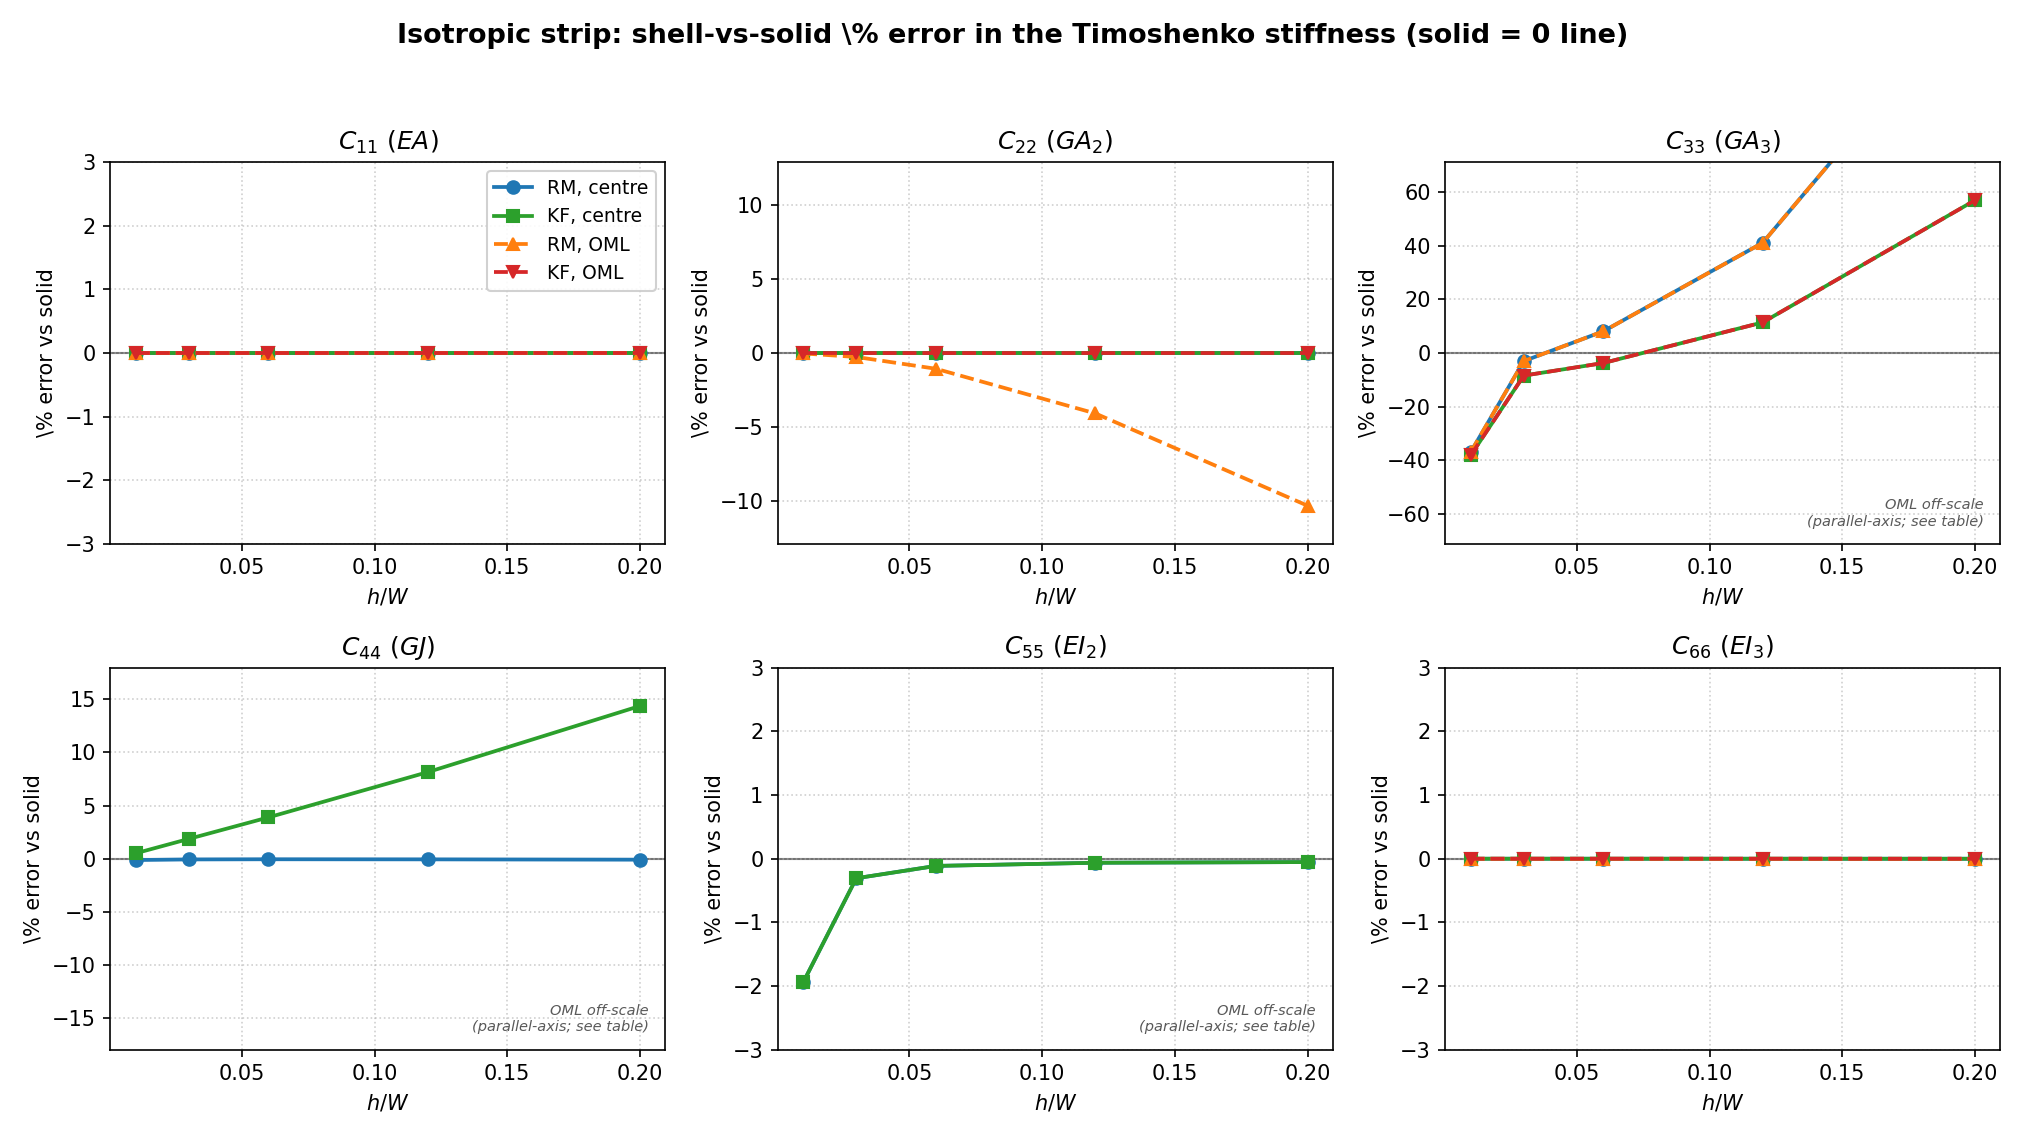
\includegraphics[width=0.49\textwidth]{err_strip_iso.png}\hfill
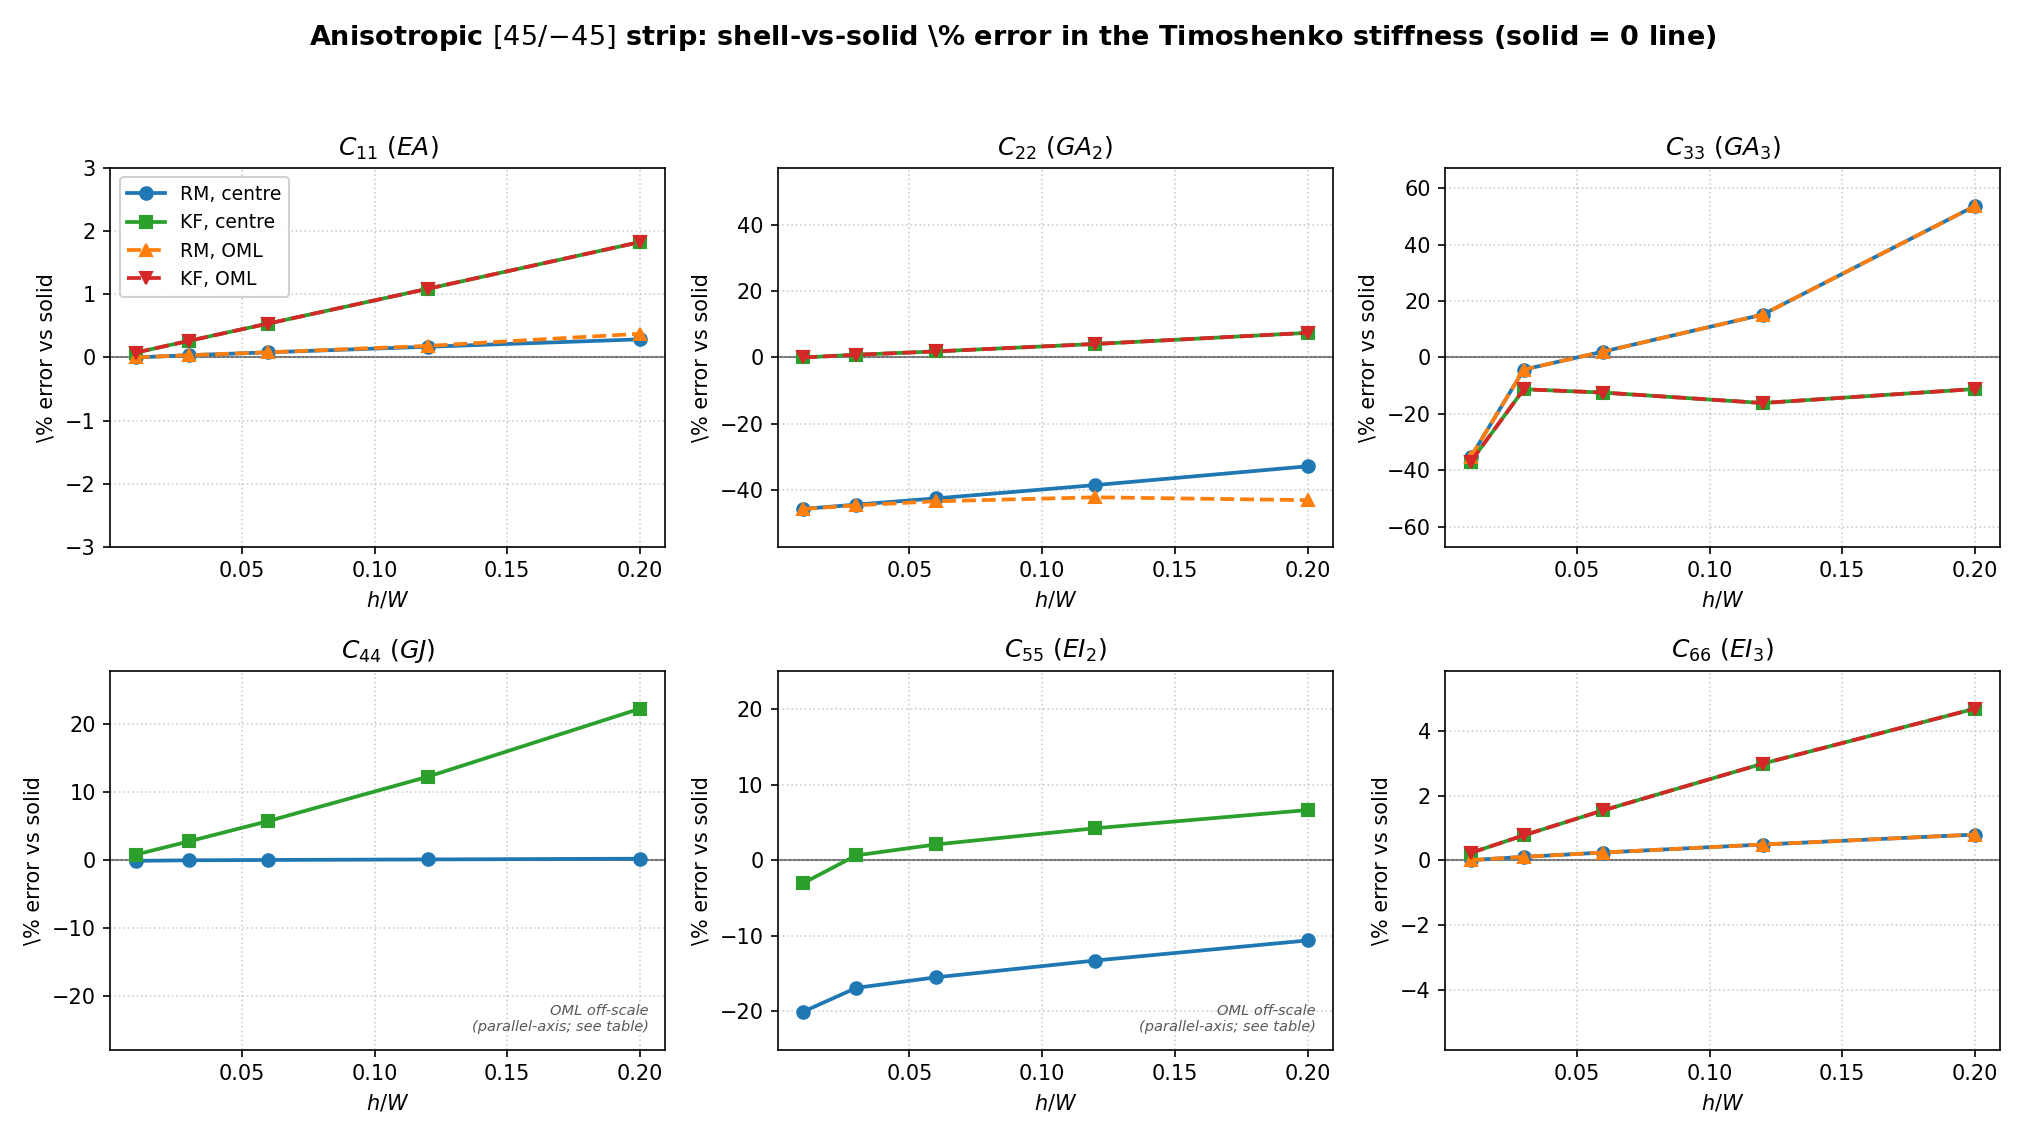
\includegraphics[width=0.49\textwidth]{err_strip_aniso.png}
\caption{Strip \% error vs.\ the solid (centre = solid lines, OML = dashed). Note
$C_{44}$ ($GJ$): RM flat at zero, KF rising---RM is more accurate for thick
open-section torsion. OML $EI_2$/$GJ$ are off-scale reference offsets.}
\end{figure}

\begin{figure}[h]\centering
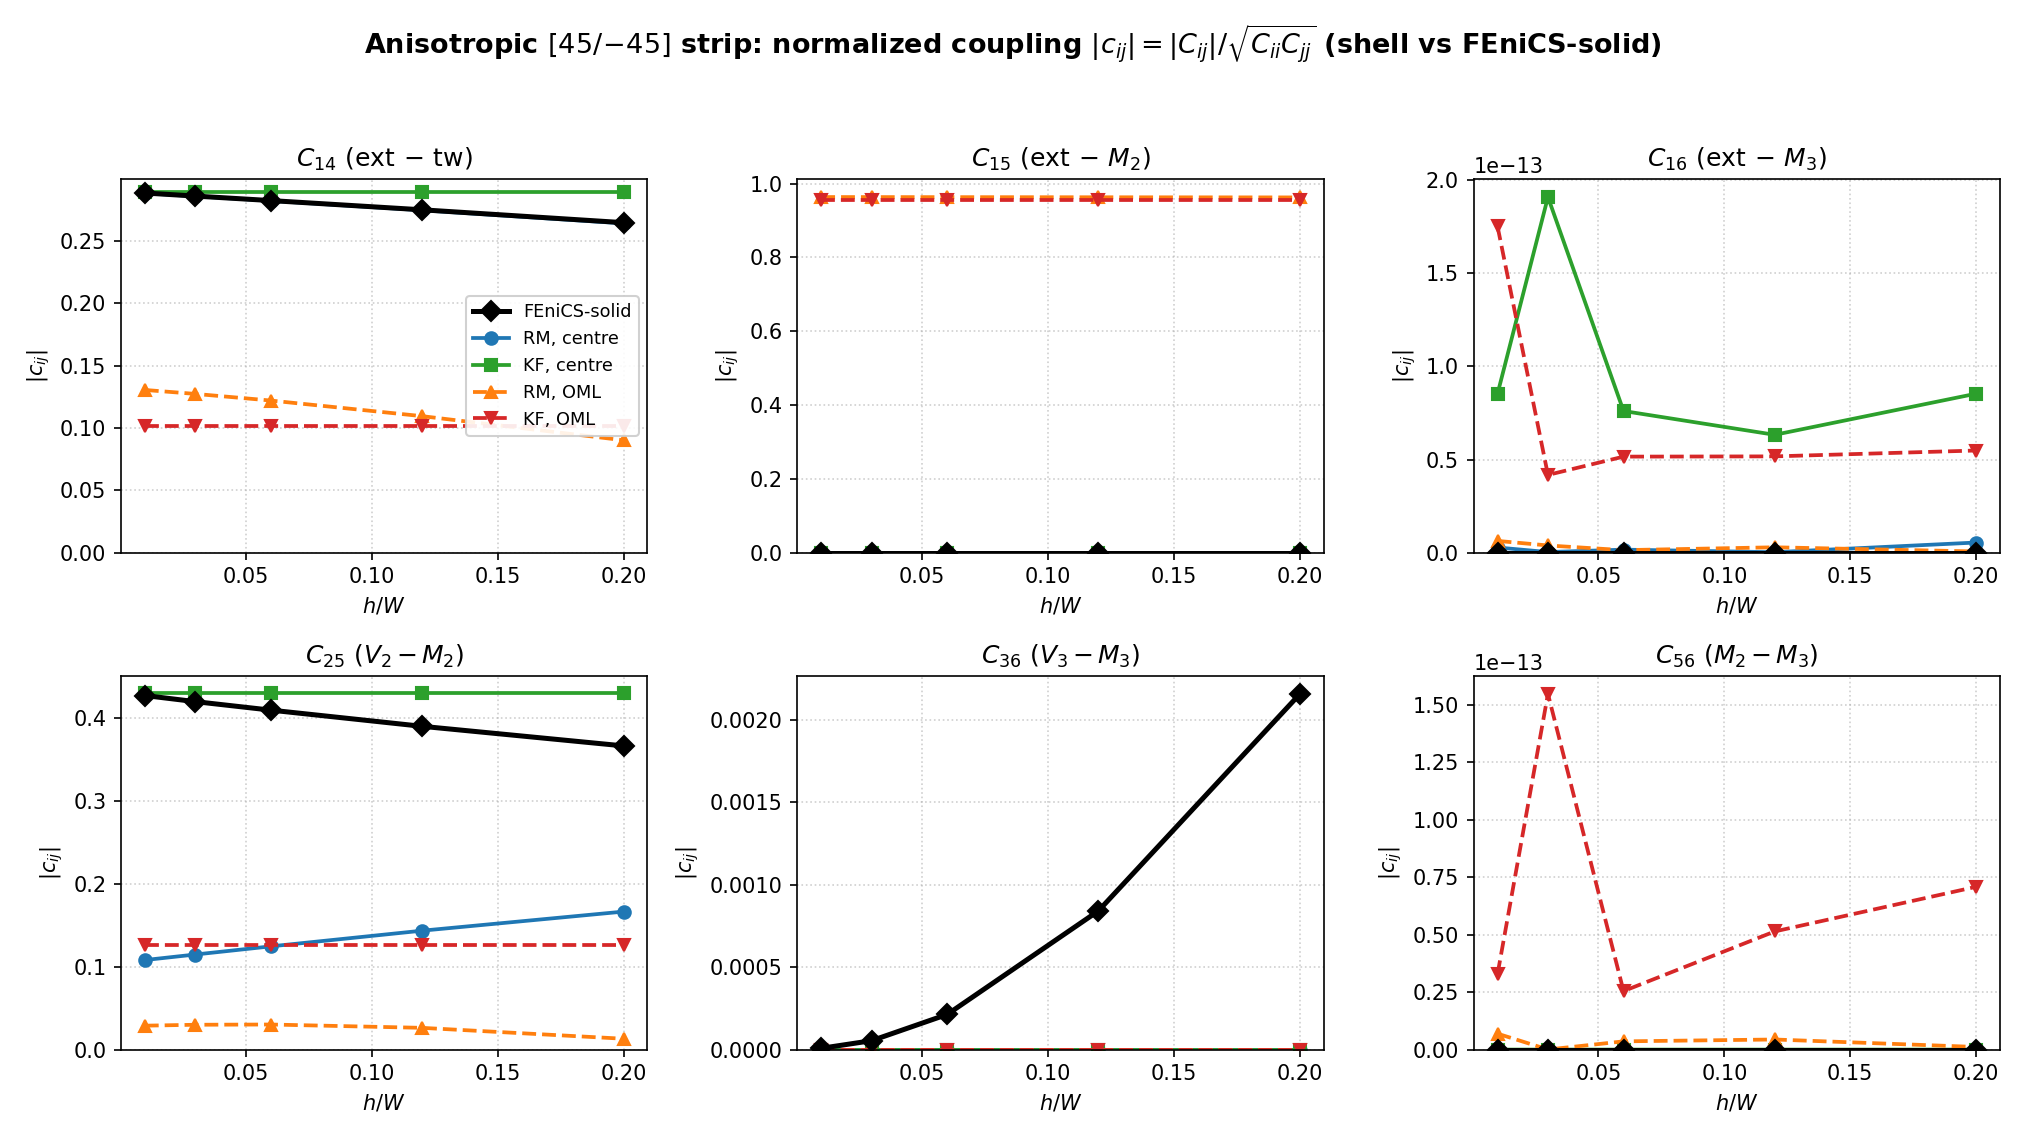
\includegraphics[width=0.49\textwidth]{coupl_strip_aniso.png}\hfill
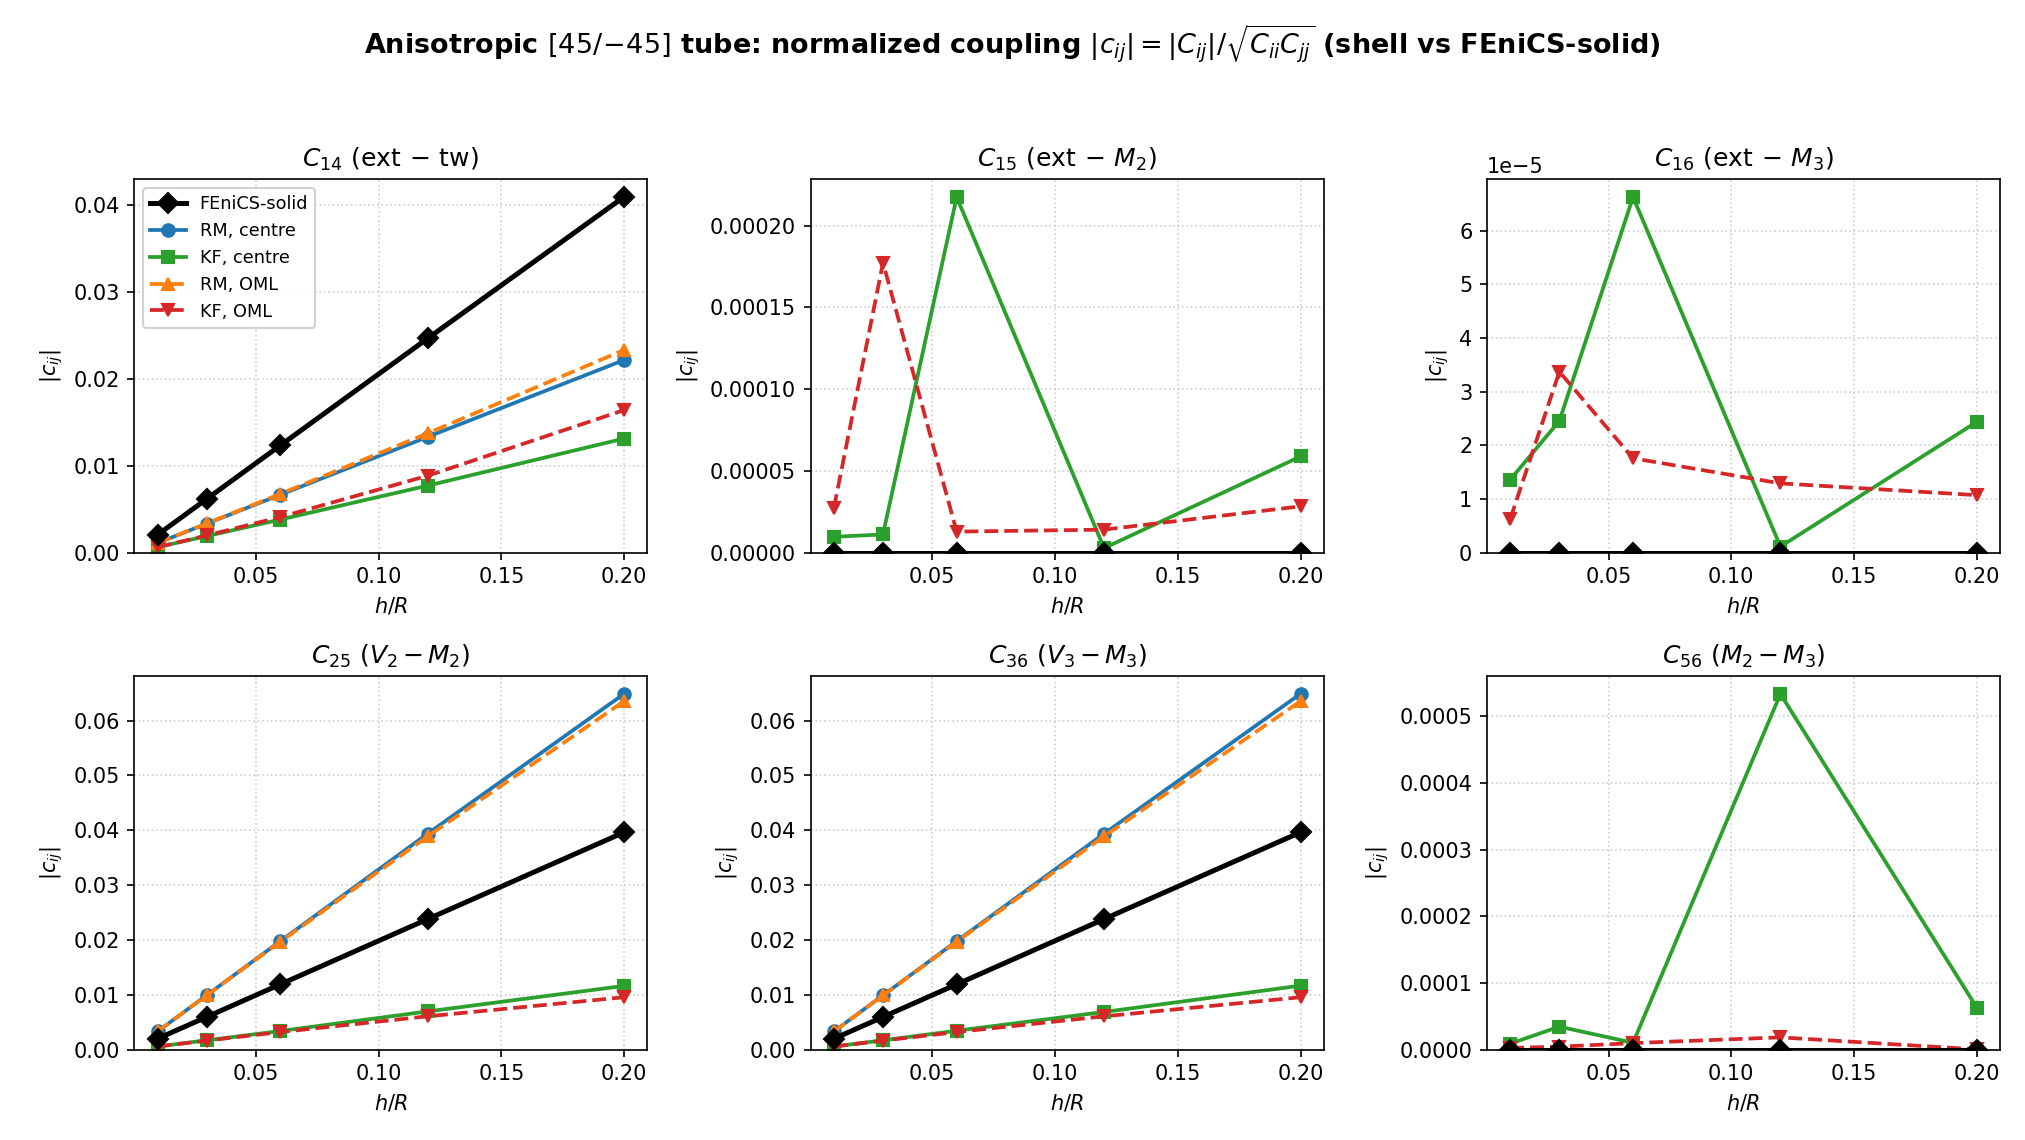
\includegraphics[width=0.49\textwidth]{coupl_tube_aniso.png}
\caption{Normalized couplings $|c_{ij}|$ for the $[45/\!-\!45]$ strip (left) and
tube (right). $C_{14},C_{25}$ are the genuine material couplings;
$C_{15},C_{16},C_{56}\approx0$ at the centre.}
\end{figure}

\paragraph{Bottom line.} Use the mid-surface reference. $EA$, $EI$ and (with the
twist correction) $GJ$ are trustworthy in both models for open and closed
sections; RM's advantage is thick-section torsion. The open-section transverse
shear ($GA$) is the remaining method-sensitive quantity. Full tables, all four
error plots, and the geometry/orientation figures are in the detailed report
(\texttt{benchmark\_report.pdf}).

\end{document}
